\section{Ley de Ohm}

Conecte el siguiente circuito indicado, empleando alambre de Nicromo
(amarillo) de diámetro $\phi = 2r = 0.75mm$.

\begin{figure}[H]
    \centering
    \begin{subfigure}[b]{0.5\textwidth}
        \centering
        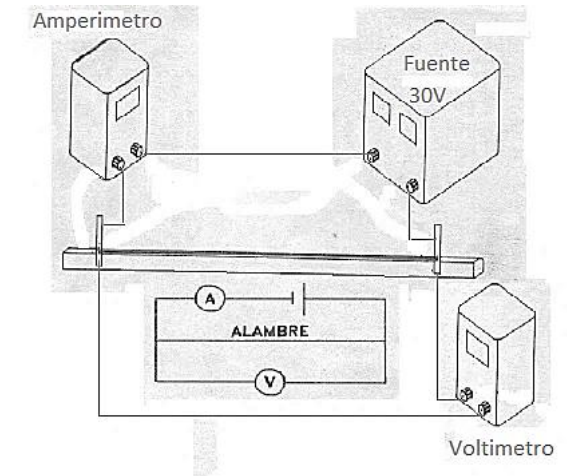
\includegraphics[width=\textwidth]{Figures/0. General/figure_1_1.png}
        \caption{\textit{Montaje Circuito 1}}
        \label{fig: Montaje Circuito 1}
    \end{subfigure}
\end{figure}

% TODO

Por lo que lo montamos de la siguiente manera:

\begin{figure}[H]
    \centering
    \begin{subfigure}[b]{0.8\textwidth}
        \centering
        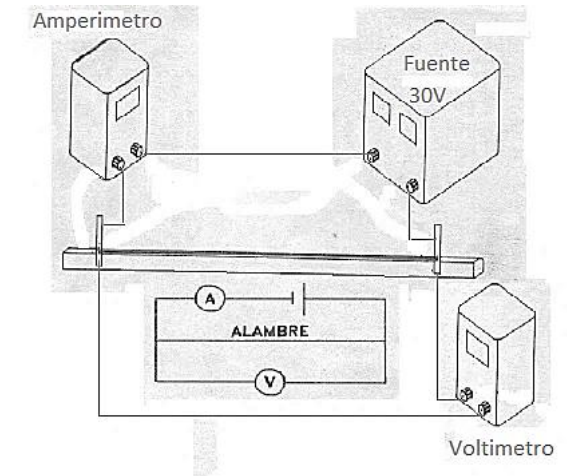
\includegraphics[width=\textwidth]{Figures/0. General/figure_1_1.png}
        \caption{\textit{Montaje Físico Circuito 1}}
        \label{fig: Montaje Fisico Circuito 1}
    \end{subfigure}
\end{figure}

\section{Constantán}
Para el alambre de Constantán (rojo) de diámetro $\Phi = 2r = 0.4m$.

\subsection{Obtención de datos}
Ajuste el voltaje de la fuente de alimentación en $1.0$ voltio y haga
lecturas de voltaje y corriente, de acuerdo a la siguiente tabla:

\subsection{$\Delta V$ vs $i(A)$}
Graficar $\Delta V$ vs $i(A)$. Encuentre la pendiente con sus respectivas
unidades.

\subsection{Calcular el error}
Calcule el porcentaje de error de la resistencia experimental encontrada en el
numeral \textit{2.2}. respecto a la resistencia teórica dada por el fabricante
$R_{T}$.


